\documentclass[12pt,a4paper,answers]{exam} % Canvia 'answers' a 'noanswers' per amagar les solucions
\usepackage[utf8]{inputenc}
\usepackage[catalan]{babel}
\usepackage{graphicx}
\usepackage{geometry}
\usepackage{fancyhdr}
\usepackage{tabularx}
\usepackage{lastpage}
\usepackage{enumitem}
\usepackage{amsmath}
\usepackage{amssymb}

% 1. MARGES I CAPÇALERA
\geometry{top=4cm, bottom=3cm, left=2cm, right=2cm, headheight=2.5cm}

\pagestyle{fancy}
\fancyhf{}
\fancyhead[L]{Trigonometria, vectors i rectes} 
\fancyhead[R]{10\% NOTA 3r T}

\fancyfoot[L]{}
\fancyfoot[C]{Pàgina \thepage\ de \pageref{LastPage}}
\fancyfoot[R]{}

\renewcommand{\headrulewidth}{0.4pt}

% Configuració de l'entorn solution per la classe exam
\shadedsolutions
\renewcommand{\solutiontitle}{\noindent\textbf{Solució:}\enspace}

\begin{document}

% --- CAPÇALERA D'IDENTIFICACIÓ ---
\begingroup
\renewcommand{\arraystretch}{2.2}
\begin{tabularx}{\textwidth}{|X|p{4cm}|}
    \hline
    \textbf{Nom i cognoms:} & \textbf{Grup:} \\ \hline
    \textbf{Exercicis trigonometria, vectors i rectes} & \textbf{Data:} \\ \hline
\end{tabularx}
\endgroup

\vspace{0.5cm}

% --- EXERCICIS ---
\begin{questions}

    % EXERCICI 1
    \question Els components d'un vector $\vec{v}$ en la base $B=\{(-3,4),(1,-2)\}$ són $(4,3)$.
    \begin{parts}
        \part Quines són les components d'aquest vector en la base canònica?
        \part I en la base $B^{\prime}=\{(1,-1),(3,2)\}$?
    \end{parts}

    \begin{solution}
        \textbf{a)} Multipliquem els components per la base $B$: 
        $\vec{v} = 4 \cdot (-3, 4) + 3 \cdot (1, -2) = (-12, 16) + (3, -6) = (-9, 10)$.
        
        \textbf{b)} Busquem $(x, y)$ tals que $(-9, 10) = x(1, -1) + y(3, 2)$:
        \[ \begin{cases} x + 3y = -9 \\ -x + 2y = 10 \end{cases} \]
        Sumant les dues equacions: $5y = 1 \implies y = 1/5$.
        Substituint a la primera: $x + 3(1/5) = -9 \implies x = -9 - 3/5 = -48/5$.
        Solució: $\vec{v}_{B'} = (-48/5, 1/5)$.
    \end{solution}

    % EXERCICI 2
    \question Considera els punts $A(-6,-4)$, $B(1,-3)$, $C(6,2)$ i $D(p,q)$.
    \begin{parts}
        \part Calcula $p$ i $q$ perquè el quadrilàter de vèrtexs els punts $ABCD$ sigui un paral·lelogram.
        \part Prova que aquest paral·lelogram té els costats iguals. De quin tipus de paral·lelogram es tracta?
        \part Calcula'n el perímetre i l'àrea.
    \end{parts}

    \begin{solution}
        \textbf{a)} S'ha de complir que el vector $\vec{AB}$ sigui igual al vector $\vec{DC}$.
        $\vec{AB} = (1 - (-6), -3 - (-4)) = (7, 1)$.
        $\vec{DC} = (6 - p, 2 - q)$.
        Igualem components: $6 - p = 7 \implies p = -1$; $2 - q = 1 \implies q = 1$. Per tant, $D(-1, 1)$.
        
        \textbf{b)} Calculem la longitud dels costats adjacents:
        $|\vec{AB}| = \sqrt{7^2 + 1^2} = \sqrt{50} = 5\sqrt{2}$.
        $\vec{BC} = (6-1, 2-(-3)) = (5, 5) \implies |\vec{BC}| = \sqrt{5^2 + 5^2} = \sqrt{50} = 5\sqrt{2}$.
        Com que tots els costats són iguals però els vectors no són perpendiculars (producte escalar $\vec{AB} \cdot \vec{BC} = 35 + 5 \neq 0$), es tracta d'un \textbf{rombe}.
        
        \textbf{c)} Perímetre: $4 \cdot 5\sqrt{2} = 20\sqrt{2} \approx 28,28$ u.
        Àrea del rombe: $A = \frac{D \cdot d}{2}$. Les diagonals són els vectors $\vec{AC}$ i $\vec{BD}$.
        $\vec{AC} = (6 - (-6), 2 - (-4)) = (12, 6) \implies D = \sqrt{12^2 + 6^2} = \sqrt{180} = 6\sqrt{5}$.
        $\vec{BD} = (-1 - 1, 1 - (-3)) = (-2, 4) \implies d = \sqrt{(-2)^2 + 4^2} = \sqrt{20} = 2\sqrt{5}$.
        Àrea = $\frac{6\sqrt{5} \cdot 2\sqrt{5}}{2} = \frac{60}{2} = 30$ $u^2$.
    \end{solution}

    % EXERCICI 3
    \question Considera la recta $r$ d'equació $3x-5y+2=0$. Esbrina les equacions de les rectes paral·lela i perpendicular que passen pel punt $(-15, 4)$.

    \begin{solution}
        La recta $r$ té com a vector normal $\vec{n} = (3, -5)$.
        \textbf{Recta paral·lela:} Té el mateix vector normal. L'equació serà $3x - 5y + C = 0$.
        Imposem que passi per $(-15, 4)$: $3(-15) - 5(4) + C = 0 \implies -45 - 20 + C = 0 \implies C = 65$.
        Equació paral·lela: $3x - 5y + 65 = 0$.
        
        \textbf{Recta perpendicular:} Intercanviem coeficients i canviem un signe. El vector normal serà $(5, 3)$. L'equació serà $5x + 3y + C' = 0$.
        Imposem que passi per $(-15, 4)$: $5(-15) + 3(4) + C' = 0 \implies -75 + 12 + C' = 0 \implies C' = 63$.
        Equació perpendicular: $5x + 3y + 63 = 0$.
    \end{solution}

    % EXERCICI 4
    \question Representa gràficament les rectes $s: 3x-y-1=0$ i $t: x+3y-12=0$.
    \begin{parts}
        \part Demostra que són perpendiculars.
        \part Calcula'n el punt d'intersecció.
        \part Determina l'àrea del triangle que limiten aquestes rectes i l'eix d'ordenades.
    \end{parts}

    \begin{solution}
        \textbf{a)} Els vectors directors són $\vec{v_s} = (1, 3)$ i $\vec{v_t} = (-3, 1)$. 
        El seu producte escalar és: $1 \cdot (-3) + 3 \cdot 1 = -3 + 3 = 0$. Per tant, són perpendiculars.
        
        \textbf{b)} Resolem el sistema: 
        De la primera equació, $y = 3x - 1$. 
        Substituïm a la segona: $x + 3(3x - 1) - 12 = 0 \implies x + 9x - 3 - 12 = 0 \implies 10x = 15 \implies x = 1,5$.
        Calculem $y$: $y = 3(1,5) - 1 = 4,5 - 1 = 3,5$.
        Punt d'intersecció: $P(1,5 \,;\, 3,5)$.
        
        \textbf{c)} Calculem els punts de tall amb l'eix d'ordenades ($x=0$):
        En $s$: $3(0) - y - 1 = 0 \implies y = -1$. Punt $A(0, -1)$.
        En $t$: $0 + 3y - 12 = 0 \implies 3y = 12 \implies y = 4$. Punt $B(0, 4)$.
        Agafem com a base del triangle el segment de l'eix Y, de $-1$ a $4$: base $b = 4 - (-1) = 5$.
        L'altura del triangle respecte aquesta base és la coordenada $x$ del punt d'intersecció: $h = 1,5$.
        Àrea = $\frac{b \cdot h}{2} = \frac{5 \cdot 1,5}{2} = 3,75$ $u^2$.
    \end{solution}

    % EXERCICI 5
    \question Si $\tan \theta=2,4$ i és un angle del 3r quadrant, calcular les altres raons trigonomètriques: $\sin \theta$, $\cos \theta$, $\sec \theta$, $\csc \theta$ i $\cot \theta$ a partir de $\tan \theta$ sense necessitat de calcular l'angle.

    \begin{solution}
        Al 3r quadrant, el sinus i el cosinus són negatius. Convertim $2,4$ a fracció: $\tan \theta = 24/10 = 12/5$.
        Utilitzem la identitat: $1 + \tan^2 \theta = \sec^2 \theta$.
        $1 + \left(\frac{12}{5}\right)^2 = 1 + \frac{144}{25} = \frac{169}{25} = \sec^2 \theta$.
        Com que estem al 3r quadrant, $\sec \theta$ és negativa: $\sec \theta = -\sqrt{\frac{169}{25}} = -\frac{13}{5}$.
        D'aquí, $\cos \theta = \frac{1}{\sec \theta} = -\frac{5}{13}$.
        Utilitzant $\tan \theta = \frac{\sin \theta}{\cos \theta}$, obtenim $\sin \theta = \tan \theta \cdot \cos \theta = \frac{12}{5} \cdot \left(-\frac{5}{13}\right) = -\frac{12}{13}$.
        Llavors: $\csc \theta = \frac{1}{\sin \theta} = -\frac{13}{12}$.
        Finalment, $\cot \theta = \frac{1}{\tan \theta} = \frac{5}{12}$.
    \end{solution}

    % EXERCICI 6
    \question Resol les següents equacions trigonomètriques:
    \begin{parts}
        \part $\sqrt{2} \sin{x} - 1 = 0$
        \part $2\cos x + \sqrt{3} = 0$
        \part $\tan^2 x - 3 = 0$
        \part $4\sin^2 x - 1 = 0$
    \end{parts}

    \begin{solution}
        \textbf{a)} $\sin x = \frac{1}{\sqrt{2}} = \frac{\sqrt{2}}{2} \implies x = 45^\circ + 360^\circ k \quad \text{i} \quad x = 135^\circ + 360^\circ k$.
        
        \textbf{b)} $\cos x = -\frac{\sqrt{3}}{2} \implies x = 150^\circ + 360^\circ k \quad \text{i} \quad x = 210^\circ + 360^\circ k$.
        
        \textbf{c)} $\tan^2 x = 3 \implies \tan x = \pm\sqrt{3}$.
        Si $\tan x = \sqrt{3} \implies x = 60^\circ + 180^\circ k$.
        Si $\tan x = -\sqrt{3} \implies x = 120^\circ + 180^\circ k$.
        (Alternativament: $x = 60^\circ + 180^\circ k$ i $x = -60^\circ + 180^\circ k$).
        
        \textbf{d)} $\sin^2 x = \frac{1}{4} \implies \sin x = \pm\frac{1}{2}$.
        Si $\sin x = \frac{1}{2} \implies x = 30^\circ + 360^\circ k \quad \text{i} \quad x = 150^\circ + 360^\circ k$.
        Si $\sin x = -\frac{1}{2} \implies x = 210^\circ + 360^\circ k \quad \text{i} \quad x = 330^\circ + 360^\circ k$.
        Es pot resumir com $x = 30^\circ + 180^\circ k$ i $x = 150^\circ + 180^\circ k$.
    \end{solution}

    % EXERCICI 7
    \question Demostra les següents igualtats trigonomètriques:
    \begin{parts}
        \part $\displaystyle \frac{1}{1+\sin\alpha}+\frac{1}{1-\sin\alpha}=2\sec^{2}\alpha$
        \part $\cos^{4}\alpha-\sin^{4}\alpha=\cos^{2}\alpha-\sin^{2}\alpha$
    \end{parts}

    \begin{solution}
        \textbf{a)} Fem el denominador comú:
        \[ \frac{1 \cdot (1-\sin\alpha) + 1 \cdot (1+\sin\alpha)}{(1+\sin\alpha)(1-\sin\alpha)} = \frac{1 - \sin\alpha + 1 + \sin\alpha}{1 - \sin^2\alpha} \]
        Simplifiquem el numerador ($1+1=2$, s'anul·la el sinus) i apliquem la identitat fonamental al denominador ($\cos^2\alpha = 1 - \sin^2\alpha$):
        \[ \frac{2}{\cos^2\alpha} = 2 \cdot \frac{1}{\cos^2\alpha} = 2\sec^2\alpha \]
        
        \textbf{b)} Considerem la part esquerra de la igualtat com una diferència de quadrats $A^2 - B^2 = (A-B)(A+B)$:
        \[ \cos^4\alpha - \sin^4\alpha = (\cos^2\alpha - \sin^2\alpha)(\cos^2\alpha + \sin^2\alpha) \]
        Com que la identitat fonamental ens diu que $\cos^2\alpha + \sin^2\alpha = 1$, ens queda:
        \[ (\cos^2\alpha - \sin^2\alpha) \cdot 1 = \cos^2\alpha - \sin^2\alpha \]
    \end{solution}

    \newpage 
    
    % EXERCICI 8
    \question Volem penjar una làmpada del sostre d'una habitació tal com mostra la figura. Si la distància entre els dos punts del sostre on se subjecta el cable és de 180 cm, es demana la longitud total de la corda i la distància respecte del sostre a què quedarà penjada la làmpada.

    \begin{center}
        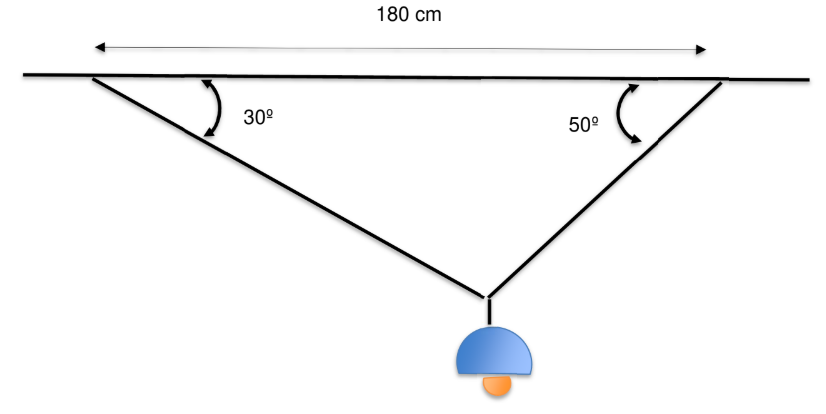
\includegraphics[width=0.6\textwidth]{imatge_lampada.png}
    \end{center}

    \begin{solution}
        Podem resoldre aquest problema aplicant el \textbf{Teorema dels Sinus}. 
        Si observem el triangle format pel sostre i els cables, tenim un costat conegut (el sostre de $180$ cm) i els dos angles adjacents de $30^\circ$ i $50^\circ$.
        L'angle on penja la làmpada (el tercer vèrtex) serà: $180^\circ - (30^\circ + 50^\circ) = 100^\circ$.
        
        Siguin $L_1$ el cable esquerre (adjunt a l'angle de $30^\circ$ i oposat al de $50^\circ$) i $L_2$ el cable dret (adjunt a l'angle de $50^\circ$ i oposat al de $30^\circ$):
        \[ \frac{180}{\sin(100^\circ)} = \frac{L_1}{\sin(50^\circ)} = \frac{L_2}{\sin(30^\circ)} \]
        
        D'aquí trobem les longituds dels dos trams de cable:
        \[ L_1 = \frac{180 \cdot \sin(50^\circ)}{\sin(100^\circ)} \approx \frac{180 \cdot 0,7660}{0,9848} \approx 140,0 \text{ cm} \]
        \[ L_2 = \frac{180 \cdot \sin(30^\circ)}{\sin(100^\circ)} = \frac{180 \cdot 0,5}{0,9848} \approx 91,4 \text{ cm} \]
        La \textbf{longitud total de la corda} és la suma dels dos: $140,0 + 91,4 = \mathbf{231,4 \text{ cm}}$.
        
        Per trobar la \textbf{distància respecte del sostre} (l'altura $h$), tracem la perpendicular i fem servir qualsevol dels dos triangles rectangles formats. Agafant el de l'esquerra:
        \[ \sin(30^\circ) = \frac{h}{L_1} \implies h = L_1 \cdot \sin(30^\circ) = 140,0 \cdot 0,5 = \mathbf{70,0 \text{ cm}} \]
        La làmpada quedarà penjada a 70 cm del sostre.
    \end{solution}

\end{questions}

% --- QUADRE RESUM ---
\newpage
\section*{Quadre Resum de Solucions}
\begin{center}
\renewcommand{\arraystretch}{1.5}
\begin{tabular}{|l|l|}
    \hline
    \textbf{Exercici} & \textbf{Resultat Final} \\ \hline
    1.a & $\vec{v}_{canonica} = (-9, 10)$ \\ \hline
    1.b & $\vec{v}_{B'} = (-48/5, 1/5)$ \\ \hline
    2.a & Punt $D = (-1, 1)$ \\ \hline
    2.b & Rombe (costats de longitud $5\sqrt{2}$) \\ \hline
    2.c & Perímetre: $20\sqrt{2}$ u; Àrea: $30$ $u^2$ \\ \hline
    3 & Paral·lela: $3x-5y+65=0$; Perpendicular: $5x+3y+63=0$ \\ \hline
    4.b & Punt d'intersecció: $(1,5 ; 3,5)$ \\ \hline
    4.c & Àrea del triangle: $3,75$ $u^2$ \\ \hline
    5 & $\sin = -\frac{12}{13}, \cos = -\frac{5}{13}, \sec = -\frac{13}{5}, \csc = -\frac{13}{12}, \cot = \frac{5}{12}$ \\ \hline
    6.a & $x = 45^\circ + 360^\circ k$ i $x = 135^\circ + 360^\circ k$ \\ \hline
    6.b & $x = 150^\circ + 360^\circ k$ i $x = 210^\circ + 360^\circ k$ \\ \hline
    6.c & $x = 60^\circ + 180^\circ k$ i $x = 120^\circ + 180^\circ k$ \\ \hline
    6.d & $x = 30^\circ + 180^\circ k$ i $x = 150^\circ + 180^\circ k$ \\ \hline
    7.a \& 7.b & \textit{Consulteu la pàgina de l'exercici per veure'n el desenvolupament} \\ \hline
    8 (Làmpada) & Altura: $70$ cm; Longitud corda total: $231,4$ cm \\ \hline
\end{tabular}
\end{center}

\end{document}